 \documentclass[letterpaper, 10pt, twocolumn, reqno]{amsart}

\usepackage{mathpazo, flushend}
\usepackage{amsmath, amsthm, amssymb, bm, enumerate, url, setspace}
\usepackage[usenames,dvipsnames,svgnames,table]{xcolor}
\usepackage[pdftex, xetex]{graphicx}
\usepackage[font={small}]{caption}
\usepackage{float, colortbl, tabularx, multirow, subcaption, environ, wrapfig, textcomp}
\usepackage[normalem]{ulem}

\usepackage{blindtext}

\usepackage[bookmarks=true]{hyperref}
%\usepackage[hyperpageref]{backref}
\hypersetup{
colorlinks=true, linkcolor=blue, citecolor=ForestGreen, filecolor=magenta, urlcolor=blue,
}
\usepackage{url, cite}

\newcommand{\pc}[2]{{\color{blue} #1}\marginpar{\tiny\noindent{\raggedright{\color{ForestGreen}[PC]}\color{brown}{ #2} \par}}}
\newcommand{\todo}[1]{{\color{gray}#1}\marginpar{\tiny\noindent{\raggedright{\color{ForestGreen}[MILD TODO]}}}}

%\newcommand{\myclearpage}{\clearpage}
\newcommand{\myclearpage}{}

% math macros
\newcommand{\abs}[1]{\ensuremath \left| #1 \right|}
\newcommand{\norm}[1]{\ensuremath \lVert#1\rVert}
\newcommand{\given}{\, \vert \,}
\providecommand{\cal}[1]{\ensuremath \mathcal{#1}}
\newcommand{\ag}[1]{\ensuremath \left\langle#1\right\rangle}
\providecommand\bigo{O}
\providecommand\smallo{o}

% shorcuts
\newcommand{\aeq}[1]{\begin{align} #1 \end{align}}
\newcommand{\aeqs}[1]{\begin{align*} #1 \end{align*}}
\newcommand{\beq}[1]{\begin{equation}#1\end{equation}}
\newcommand{\beqs}[1]{\begin{equation*}#1\end{equation*}}
\newcommand{\trm}[1]{\ensuremath \textrm{#1}}
\newcommand{\enum}[2]{\begin{enumerate}[#1]{#2}\end{enumerate}}
\newcommand{\clist}[1]{\begin{itemize}\setlength{\itemsep}{0pt}
\setlength{\parsep}{0pt}
{#1}\end{itemize}}
\newcommand{\bmat}[1]{\begin{bmatrix}#1\end{bmatrix}}
\newcommand{\mpage}[2]{\begin{center}
\begin{minipage}{#1}#2\end{minipage}\end{center}}
\newcommand{\la}{\leftarrow}
\newcommand{\ra}{\rightarrow}
\providecommand\f[2]{\ensuremath \frac{#1}{#2}}
\providecommand\rbrac[1]{\ensuremath \left(#1\right)}
\providecommand\sqbrac[1]{\ensuremath \left[#1\right]}
\providecommand\cbrac[1]{\ensuremath \left\{#1\right\}}

\newtheorem{theorem}{Theorem}
\newtheorem{proposition}[theorem]{Proposition}
\newtheorem{lemma}[theorem]{Lemma}
\newtheorem{corollary}[theorem]{Corollary}
\newtheorem{problem}[theorem]{Problem}

\theoremstyle{definition}
\newtheorem{definition}[theorem]{Definition}
\newtheorem{example}[theorem]{Example}
\newtheorem{note}[theorem]{Note}
\newtheorem{remark}[theorem]{Remark}

\newtheorem{assumption}[theorem]{Assumption}
\providecommand{\qed}{\hfill \mbox{\raggedright \rule{0.1in}{0.1in} } }

% gray proof
\let\myoldproof=\proof
\let\myoldendproof=\endproof
\renewenvironment{proof}
{\myoldproof\color{gray}}
{\myoldendproof}

% notation
\renewcommand{\P}{\trm{P}}
\newcommand{\E}{\trm{E}}
\providecommand{\ones}{\mathbb{1}}
\providecommand{\ind}{{\bf 1}}
\providecommand{\SAT}{\trm{SAT}}
\providecommand{\NAESAT}{\trm{NAE-SAT}}
\providecommand\sat{\models}
\providecommand\ksat{k\trm{-SAT}}
\providecommand\n[1]{\overline{#1}}
\providecommand{\oor}{\vee}
\providecommand{\aand}{\wedge}
%\providecommand{\implies}{\rightarrow}
\renewcommand{\sf}{S(F)}
\renewcommand{\sc}{S(c)}
\providecommand\s{\sigma}
\renewcommand{\t}{\tau}
\renewcommand{\a}{\alpha}
\renewcommand{\b}{\beta}
\renewcommand{\L}{\Lambda}
\renewcommand{\l}{\lambda}

\newcommand{\wsf}{w(\s,F)}
\newcommand{\lsf}{L(\s,F)}
\newcommand{\wsc}{w(\s,c)}
\newcommand{\wv}{w(v)}
\newcommand{\wu}{w(u)}
\newcommand{\wtf}{w(\t,F)}
\newcommand{\wtc}{w(\t,c)}
\newcommand{\puva}{\Phi_{u,v}(\a)}

\usepackage[margin=0.75in]{geometry}
\linespread{1.05}

% \usepackage[marginal]{showlabels}
% \renewcommand{\showlabelfont}{\footnotesize\slshape\color{brown}}

\newcommand{\algsize}{\footnotesize}
\setlength{\floatsep}{0.0in}
\setlength{\textfloatsep}{0.0in}
\setlength{\intextsep}{0.0in}
\setlength{\belowcaptionskip}{0.05in}
\setlength{\abovecaptionskip}{0.05in}
\setlength{\abovedisplayskip}{0.05in}
\setlength{\belowdisplayskip}{0.05in}

\graphicspath{{../fig/}}

\title{Phase transitions in random $k$-SAT}
\author{Pratik Chaudhari$^*$}
\thanks{$^*$ Laboratory of Information and Decision Systems, MIT.\newline
Email: \href{pratik.ac@gmail.com}{pratik.ac@gmail.com}}
\date{May 3, 2014}

\begin{document}
\maketitle
{\small
\textbf{\emph{Abstract:}}
This project discuses bounds for sharp transition thresholds in random satisfiability problems using the second moment method. We look at bounds for random $k-\SAT$ formulas and motivate the structure of the solution space using these arguments. Next, we briefly discuss the phenomenon of ``dynamical phase transition'', i.e., phase transition into a ``glassy'' state wherein, the solution space is clustered into exponentially many small clusters. The glassy phase has been a major bottleneck for naive ``local'' algorithms for satisfiability.
}

\section{Introduction}
\label{sec:intro}
It has become increasingly apparent that phenomenon in statistical physics such as phase transitions and glassy phases have a strong bearing on important problems in computer science and information theory such as satisfiability, error correcting codes etc. Realizing that extreme slowdown in algorithms for these problems and glassy phase transitions occur hand in hand is interesting both theoretically, and also promises to provide insights into faster, more efficient algorithms. This has spurred interest in ideas from statistical physics such as ``replica symmetry'' and ``cavity method'', which are the basis of state-of-the-art algorithms like survey propagation. Let us note that these concepts have also triggered development in the compressed sensing literature, e.g, \cite{krzakala2012statistical}.

%On a related note, the same concepts have also triggered development in the compressed sensing literature. The theoretical limit for the ratio of the number of measurements $m$ needed to recover an $n$-dimensional signal is its sparsity ratio. Message passing algorithms based on L1 minimization cannot reach this limit and it turns out that there exists a sharp threshold when the solution phase


Motivated by these results, we look at phase transitions in random $\ksat$ problems. We will use the second moment method to obtain bounds for clause
densities at which $\ksat$ becomes unsatisfiable with high probability. This is however not very illuminative, it was noticed that a number of (randomized)
polynomial time algorithms do not work close to the satisfiability threshold. Towards this end, we will also discuss dynamical phase transition, which is
when the solution space of $\ksat$ changes drastically --- it goes from looking like a giant ball to the ``error correcting code'' regime. We will discuss major ideas driving this work and sketch proofs for these results. Let us first introduce the problem setup for random $\ksat$.

\section{Setup}
\label{sec:setup}
A $k$-clause is a disjunction of $k$ Boolean variables, given $n$ Boolean
variables, a random $k$-CNF formula, $F_k(n, m)$ is formed by conjunction of $m = rn$ such $k$-clauses, selected uniformly and independently with
replacement from the set of all $k$-clauses on these $n$ variables. We assume that all formulas are in conditional normal form (CNF) and call this model ``random $\ksat$''. Let $\SAT$ be the set of all satisfiable formulas. Also,
let $r_k = \sup \{ r: F_k(n, rm) \in \SAT \}$ and $r_k^* = \inf \{ r: F_k(n, rn) \not\in \SAT \}$. Note that we always talk of $F_k(n,rn) \in \SAT$ with high probability, i.e., $\lim_{n\to \infty} \P(F_k(n,rn) \in \SAT) = 1$ if $r < r_k$.

Note that $r_k < r_k^*$ and in Sec.~\ref{sec:sat_thresh}
we will show that, in fact, $r_k = r_k^*(1-\smallo(1))$. We will also show that for $k > 22$,
\beq{
r_k \geq 2^k \log2 - (k+1)\f{\log2}{2} - \bigo(1).
\label{eqn:r_k_exact}
}

\section{Satisfiability thresholds}
\label{sec:sat_thresh}


\subsection{2-SAT}
\label{ssec:2sat}
2-SAT has a special structure, observe that $\n{x_1} \oor x_2$ is equivalent to $x_1 \implies x_2$. Given $F_2(n, rn)$, construct a graph with
vertices $x_1, \n{x_1}, x_2, \ldots, \n{x_n}$ and draw two edges, $(x_1, x_2)$ and $(\n{x_2}, \n{x_1})$ for every clause of the form $\n{x_1} \oor x_2$. It can be shown that $F_2(n,rn) \notin \SAT$ iff
there exists a path from some $x_k$ to $\n{x_k}$ and from $\n{x_k}$ to $x_k$, i.e., a bicycle. Indeed, if $\s$ satisfies $x_k$, then by following the implications in this bicycle,
we get that $\s$ satisfies $\n{x_k}$ as well and vice-versa. Also, if there does not exist a bicycle and the formula is not $\SAT$, we can simply set one of the
variables to 1 and follow the implications; we can keep doing this because there are no bicycles, and we arrive at a solution of $F_2(n, rn)$. So the
assumption that $F_2(n,rn) \in \SAT$ has to be false.

Let the length of this bicycle be $s$ if some path
$$(u, w_1, w_2, \ldots, w_s, v)$$
with $u,v \in \{w_1, \ldots, w_s,\n{w_1}, \ldots, \n{w_s}\}$
exists. The probability of this happening, by Markov's inequality, is
$$
\P(F_2(n,rn) \notin \SAT) \leq \sum_{s=2}^n \binom{n}{s} s^2 (2s)^2 \binom{m}{s+1} \rbrac{\f{1}{4 \binom{n}{2}}}^{s+1}.
$$
By direct summation, it is easy to see that this is $\bigo(1/n)$ iff $r <1$, i.e., $r_2^* < 1$. This was an example of the first moment method. Using the second moment method, similar to Sec.~\ref{ssec:ksat_weighted}, we can get $r_2 > 1$, i.e., the phase transition threshold is simply $r = 1$. We do this by counting the number of snakes, i.e., cycles where $u = \n{v}$ and $u \in \cbrac{w_1, \ldots, w_s}$. Note the nature of this analysis, to make the second moment work, we have to resort to consider only a subset of all bicycles.

\subsection{Vanilla second moment method}
\label{ssec:ksat_vanilla}
To get a ball-park estimate, let us compute a simple upper bound for the phase
transition. The number of all possible $k$-clauses is $C_k = 2^k \binom{n}{k}$
 while the number of clauses satisfied by a given random assignment is $S_k = (2^k -1) \binom{n}{k}$. Thus the probability of $F \in \SAT$ is $\binom{S_k}{m}/\binom{C_k}{m} < (1-2^{-k})^m$, which means that the expected number of
satisfying assignments is $2^n (1-2^{-k})^{rn} = \smallo(1)$ for $r > 2^k \log 2$ which implies $r_k^* < 2^k \log 2$.

The idea behind the rest of this section is to get a non-zero lower bound in the limit for $P(X > 0)$, where $X$ is the number of solutions of random $\ksat$. We can then use Chebyshev's inequality, $P(X>0) \geq \E[X]^2/\E[X^2]$. It is however instructive to note that we cannot weigh each satisfying assignment equally, the bounds are too loose that way. Let us review why.

For a random formula $F$, let $\sf$ be the set of satisfying assignments and let $X = \abs{\sf}$. If $F = c_1 \aand c_2 \ldots c_m$, we have
\aeq{
\E[X^2] &= \E\sqbrac{\rbrac{\sum_\s \ind_{\s \in \sf}}^2} &&= \E\sqbrac{\sum_{\s,\t} \ind_{\s,\t \in \sf}} \notag \\
&= \sum_{\s,\t} \E \sqbrac{\prod_c \ind_{\s,\t \in \sc}} &&= \sum_{\s,\t} \prod_c \E[\ind_{\s,\t \in \sc}].
\label{eqn:calc_x2}
}
We can now see that
\beq{
\P(\s,\t \in \sc) = 1 -2^{1-k} - 2^{-k}\a^k = f_s(\a)
\label{eqn:ksat_vanilla_st}
}
where $\s$ and $\t$ assign the same value to $z = \a n$ variables. This follows because if $\s \not\sat c$, the only way for $\t \not\in c$ is for all $k$ variables in $c$ to lie in the overlap. $f_S$ thus quantifies the correlation between $\s,\t$ being both satisfying assignments of $F$. We now have
$$
\E[X^2] = 2^n \sum_{z=0}^n \binom{n}{z} f_S(\a)^m,
$$
whereupon, using $\binom{n}{z} = \rbrac{\a^\a (1-\a)^{1-\a}}^{-n} poly(n)$, we have
\aeq{
\E[X^2] &\leq 2^n \rbrac{\max_{0 \leq \a \leq 1} \sqbrac{ \f{f_S(\a)^r}{\a^\a (1-\a)^{1-\a}} } }^n poly(n) \notag \\
&:= \rbrac{\max_{0 \leq \a \leq 1} \L_S(\a)}^n poly(n).
\label{eqn:ksat_vaniall_second_moment}
}

At the same time, note that
$$
\E[X]^2 = \rbrac{2^n \rbrac{1 - 2^{-k}}^m }^2 = \L_S(1/2)^n,
$$
and hence if we have some $\a \in [0,1]$ with $\L_S(\a) > \L_S(1/2)$ the
the second moment is exponentially greater than the square of the first moment and hence we have an exponentially smaller lower bound on $\P(X > 0)$. In
other words, we need to reduce the contribution to $E[X^2]$ from $\s,\t$ with overlap of $\a > 1/2$; recollect that we used a similar ``snake'' counting method as opposed to just bicycles. Work on Not All Equal-SAT, i.e., every clause has at
least one satisfied and one unsatisfied literal gives some clues. For $\NAESAT$, we have
$$
\P(\s,\t \in \NAESAT) = 1 - 2^{2-k} + 2^{1-k} \rbrac{\a^k + (1-\a)^k}
$$
which is symmetric about $\a = 1/2$ and as a result, $\L_N(\a)$ has a maxima at $1/2$ for $r \leq 2^{k-1} \log2 -1$. It was shown in~\cite{achlioptas2002asymptotic} that for $r \geq 2^{k-1} \log2$, $\NAESAT$ is not satisfiable, i.e., the second moment method actually gives bounds within additive constant. We will use this as a motivation to design a weighing function on the set $\sf$. Roughly, we reduce the contribution to $\E[X^2]$ due to the correlation terms from Eqn.~\eqref{eqn:ksat_vanilla_st}.

\subsection{Weighted second moment method}
\label{ssec:ksat_weighted}
Let $\wsf$ be some weighing function and $\wsf = 0$ if $\s \notin \sf$. We assume in this section that $\wsf$ factors exactly over the clauses and define $X$ as follows.
$$X = \sum_\s \wsf = \sum_\s \prod_c \wsc.$$
This choice still works for us because if we can prove $\E[X^2] = \bigo\rbrac{\E[X]^2}$, we will have
$$\P(\abs{\sf} > 0) = \P(X > 0) \geq \f{E[X^2]}{\E[X]^2} = \bigo(1).$$
Again,
\aeqs{
\E[X]^2 &= 2^n \rbrac{\E[\wsc]}^m \\
\E[X^2] &= \sum_{\s,\t} \prod_c \E[\wsc \wtc]\\
&= \sum_{\s,\t} \rbrac{\E[\wsc \wtc]}^m
}
where the clause $c = \ell_1 \oor \ldots \oor \ell_k$ is random. We want $\wsc$ to be independent of variable labels, so let it be $\wsc = \wv$ where $v_i =1$ if $\s \sat \ell_i$ and $-1$ otherwise.

If $v \in A = \{-1,1\}^k$, since the literals are drawn uniformly and independently, we have
$$
\E[\wsc] = \sum_{v \in A} \wv 2^{-k}.
$$
Similarly for $\s, \t$ with an overlap of $z =\a n$,
\aeqs{
\E[\wsc \wtc] &= \sum_{u,v \in A} \wu \wv 2^{-k} \prod_{i=1}^k \a^{\ind_{u_i = v_i}} (1-\a)^{\ind_{u_i \neq v_i}} \\
&:= \sum_{u,v \in A} \wu \wv \puva := f_w(\a).
}
The second moment now looks like
\aeq{
\E[X^2] &= 2^n \sum_{z=0}^n \binom{n}{z} f_w(\a)^m \notag \\
&\leq 2^n \rbrac{\max_{0 \leq \a \leq 1} \sqbrac{ \f{f_w(\a)^r}{\a^\a (1-\a)^{1-\a}} } }^n poly(n) \notag \\
&:= \rbrac{\max_{0 \leq \a \leq 1} \L_w(\a)}^n poly(n),
\label{eqn:Lw}
}
with $\E[X]^2 = \L_w(1/2)^n$. There are two aspects of the above expression which will help us get $\E[X^2]/\E[X]^2 = \bigo(1)$. $\L_w(\a)$ has a global maximum at $1/2$ and the $poly(n)$ factor above is in fact, just $\bigo(1)$. The former requires that $f_w'(1/2) =0$. We thus have
\aeqs{
f_w'(\a) &= \sum_{u,v \in A} \wu \wv \puva \sqbrac{\log \puva}' \\
&= \sum_{u,v \in A} \wu \wv \puva \sum_{i=1}^k\ \rbrac{\f{\ind_{u_i = v_i}}{\a} - \f{\ind_{u_i \neq v_i}}{1-\a}} \\
2^{2k-1} f_w'(\a) &= \sum_{u,v \in A} \wu \wv u v \\
&= \rbrac{\sum_u \wu u}\rbrac{\sum_v \wv v}.
}
Therefore for any $w$, we need
\beq{
f_w'(1/2) = 0 \implies \sum_{v \in A} \wv v = 0.
\label{eqn:wv_sum}
}

It is now evident that the real reason why the calculations in Sec.~\ref{ssec:ksat_vanilla} failed was because $w_S(\cdot)$ assigns 0 to $(-1,\ldots,-1)$
and $1/(2^k-1)$ to all other vectors. On the other hand, for $\NAESAT$, $w_N(\cdot)$ assigns 0 to both $(-1,\ldots,-1)$ and $(1,\ldots,1)$ and hence satisfies Eqn.~
\eqref{eqn:wv_sum}. Hence, we shall construct such a $w(\cdot)$. In addition to this, to sharpen the results, we need to make sure that $w$ is as close $w_S
$ as possible. By a simple summation, Eqn.~\eqref{eqn:wv_sum} can also be written as
$$
\sum_{v \neq (-1,\ldots,-1)} \wv (2\abs{v} - k) = 0.
$$
where $\abs{v}$ is the number of 1s in $v$. We maximize entropy ($w_S$ is uniform and has maximum entropy) subject to this constraint to get $\wv \propto \l^{\abs{v}}$ with $\l$ satisfying $(1+\l)^{k-1} = 1/(1-\l)$.

We therefore work with a weighing function
\beq{
\wsf \propto \prod_c \l^{L(\s,F)} \ind_{\s \in \sc}
\label{eqn:ksat_weighing_function_exact}
}
where $\lsf$ is the number of literals in $F$ satisfied by $\s$. This results in the following theorem.

\begin{theorem}
There exists a sequence $\b_k \to 0$ s.t. $\forall\ k \geq 22$,
$$
r_k \geq 2^k \log 2 - 2(k+1) \log 2 - 1 - \b_k.
$$
\label{thm:bound_weighted}
\end{theorem}
\begin{remark}
Note that the second term is off by a factor of 4 as compared to Eqn.~\eqref{eqn:r_k_exact}. This is because of our constraint that $\wsf$ factors exactly over all clauses. It is possible to sharpen these bounds as shown in Sec.~\ref{ssec:sharper_bounds}. Also, in the following proof, we will neglect improper clauses, i.e., repeated or contradictory literals since their probability is at most $k^2/n$ each, i.e., w.h.p there are at most $\smallo(n)$ of them. Similarly, we also let the model select clauses with replacement since w.h.p there are at most $\smallo(n)$ clauses that contain the same $k$ variables.
\end{remark}
%
\begin{proof}[Proof Sketch] Let $\hsf$ be the number of satisfied literal occurrences in $F$ minus the number of unsatisfied literals. For $0 < \g \leq 1$, let $X = \sum_\s \g^{\hsf} \ind_{\s \in \sf}$.  Note that $\hsf = 2\lsf - k m$ and hence this is the same as Eqn.~\eqref{eqn:ksat_weighing_function_exact}. Fix $\s$ and since literals in $c = l_1 \oor \ldots \oor l_k$ are random, we have
\aeqs{
\E \sqbrac{\g^\hsc \ind_{\s \in \sf}} &= \E\sqbrac{\g^\hsc} - \E\sqbrac{\g^{-k}\ind_{\s \notin \sc}}\\
&:=\psi(\g).\\
\implies \E[X] &= (2\psi(\g)^r)^n.
}
Similarly, if $\s, \t$ overlap in $\a n$ literals, we can get
\aeq{
\E\sqbrac{\g^{\hsl + \htl}} &= \a \rbrac{\g^2 + \g^{-2}}/2 + 1 - \a \notag\\
\E\sqbrac{\g^{\hsl + \htl} \ind_{\s \notin \sc}} &= 2^{-k} (\a \g^{-2} + (1-\a)) \notag\\
\E\sqbrac{\g^{\hsl + \htl} \ind_{\s,\t \notin \sc}} &= 2^{-k} (\a \g^{-2}) \notag\\
\implies
\E\sqbrac{\g^{\hsc + \htc} \ind_{\s,\t \in \sc}} &= \f{f(\a)}{2^k(1-\e)^k}.
\label{eqn:g_st}
}
for some explicit $f(\a)$ and $\e = 1-\g^2$. Using the same calculations as in Eqn.~\eqref{eqn:calc_x2}, we now have
\beq{
\E[X^2] = 2^n \sum_{z=0}^n \binom{n}{z} \rbrac{\f{f(\a)}{2^k(1-\e)^k}}^n.
\label{eqn:x2_weighted}
}
The right hand side can be bounded by noting that only $\bigth(n^{1/2})$ of the binomial coefficients dominate, i.e., if $g = \f{f(\a)}{\a^\a + (1-\a)^{1-\a}}$,
and there exists $\a_{\max}$ s.t. $g(\a_{\max}) > g(\a)$ for all $\a \in (0,1)$ and $g''(\a_{\max}) < 0$ --- it can be shown that these conditions are true in our case for $k > 22$
$$
r < 2^k \log 2 -2 \log2(k+1) - 1 -3/k,
$$
--- then there exists $C > 0$ s.t.
$$
\E[X^2] < C\ \rbrac{\f{2 g(1/2)}{(2-2\e)^{kr}} }^n.
$$
where $\e = 1-\g^2$. Now observe that
\beq{
\E[X]^2 = \rbrac{\f{2 g(1/2)}{(2-2\e)^{kr}}}^{n}
\label{eqn:weighted_ex_explicit}
}
and the proof is complete by Chebyshev's inequality.
%--
% $$
% \P(X > 0) \geq \f{\E[X]^2}{\E[X^2]} \geq \f{1}{C}.
% $$
\end{proof}

\subsection{Sharper bounds using measure transform}
\label{ssec:sharper_bounds}

This section hunts down the missing factor of 4 in Thm.~\ref{thm:bound_weighted}. From Eqn.~\eqref{eqn:ksat_vaniall_second_moment}, we see that the dominant
contributions to $\E[X^2]$ come from pairs where fewer than half of the
literals satisfied. Hence we construct
$\spf = \cbrac{\s \in \sf: \hsf > 0}$
(cf. proof of Thm.~\ref{thm:bound_weighted}). In Lem.~\ref{lem:dyn_moments_close}, we will show that $\E[X_+]/\E[X] \to 1/2$ a.s. where $X_+ = \sum_{\s \in \spf}\ \g^\hsf$. If this is true, consider Eqn.~\ref{eqn:g_st} with some $\e = 1 -\th^2$ with $\th^2 \geq \g^2$, we have
\aeqs{
\E\sqbrac{\g^{\hsf + \htf} \ind_{\s,\t \in \spf}} &\leq \E\sqbrac{\th^{\hsf + \htf} \ind_{\s,\t \in \spf}} \\
&\leq \E\sqbrac{\g^{\hsf + \htf} \ind_{\s,\t \in \sf}}\\
&:= f_2(\a, \e)^m.
}
where $f_2(\a,\e)$ is the same as $f(\a) (2-2\e)^{-k}$ from Eqn.~\eqref{eqn:g_st}. Since this holds for any $\e \leq 1 -\g^2$, we can write for $\e_0 = 1 - \g^2$
\aeqs{
\E\sqbrac{\g^{\hsf + \htf} \ind_{\s,\t \in \spf}} &\leq \sqbrac{\inf_{\e \leq \e_0} f_2(\a, \e)}^m \\
\implies \E[X_+^2] &\leq 2^n \sum_{z=0}^n \binom{n}{z} \sqbrac{\inf_{\e \leq \e_0} f_2(\a, \e)}^m
}
Again truncate the binomial coefficients and note that from Lem.~\ref{lem:dyn_moments_close} and Eqn.~\eqref{eqn:weighted_ex_explicit}, we have
$$
5 \E[X_+^2] > \E[X]^2 = g(1/2, \e_0)^n.
$$
If we can now find a piecewise constant function $\xi$ such that $g(1/2,\e_0) > f_2(\a,\xi(\e))/(\a^\a + (1-\a)^{1-\a})$ we can again apply Chebyshev's inequality to each of the piecewise constant pieces to get $\P(X_+ > 0)$ with a new bound
\beq{
r_k > 2^k \log 2 -\f{\log 2}{2} (k+1) -1 -50k^3 2^{-k}.
\label{eqn:threshold_exact_form}
}
Please see Lem.~9 in~\cite{achlioptas2004threshold} for a proof of this idea.

\begin{lemma}
For some $\g$, as $n\to \infty$, we have $\f{\E[X_+]}{\E[X]} \to 1/2$.
\label{lem:dyn_moments_close}
\end{lemma}
\begin{proof}
This is proved by a classic measure tilting argument. Let $\bP$ be the probability assigned to a sequence of random literals that form $F$, i.e., $l_1, \ldots, l_{km}$. Tilt this measure to ensure $\E_\g[\hsc\ \ind_{\s \in \sc}] = 0$ by using
$$
\bPg[\hsl = 1] = \f{\g}{\g + \g^{-1}} = \f{2 \g}{\g + \g^{-1}} \bP[\hsl = 1].
$$
Because literals are independent, for a clause $c$, we have
$$
\bPg(c) = \f{2^k \g^{\hsc} \bP(c)}{(\g +\g^{-1})^k}.
$$
Define a new measure $\btPg(c) \propto \bPg(c)\ \ind_{\s \in \sc}$. A random formula $F$ will be sampled from this measure with probability
$$
\bPg(F) \propto \g^{\hsf}\ \P(F)\ \ind_{\s \in \sf}
$$
and since we have again have $\tilde{\E}_\g[\hsc] = 0$, we get
$$
\btPg[\hsf \geq 0] \to 1/2.
$$
Use the definition of $X, X_+$ to prove the claim.
\end{proof}


\section{Dynamical phase transition}
\label{sec:dynamical_transition}

In this section, we describe a few results on the geometry of the solution space of random $\ksat$. The motivation for these results comes from the following --- a very simple algorithm can find satisfying assignments for $r = \bigo(2^k/k)$ with
high probability~\cite{chao1986probabilistic}, it simply assigns a random value to a randomly unassigned variable and simplifies the clauses. In fact an algorithm based on belief
propagation can solve instances up to $r = \bigth(2^k \f{\log k}{k})$ using an idea known as decimation \cite{montanari2007solving}. However, in Sec.~\ref{sec:sat_thresh}, we saw that $\ksat$ is satisfiable for far more after that; it has solutions (w.h.p) until $r = 2^k \log 2 - O(k)$. This apparent discrepancy can
be resolved with the following theorem towards which we work in this section.

It turns out that the solution space, i.e., $\sf$ looks like a giant ball
until $r = \bigo(2^k/k)$ and shatters into exponentially many clusters with
exponentially small number of solutions in each as $r$ increases. We will use the Hamming distance between two satisfying instances $\s,\t$ and say that they are adjacent if $\abs{\s-\t} = 1$. A region is then the union of connected components of $\sf$.

\begin{figure}[H]
\centering
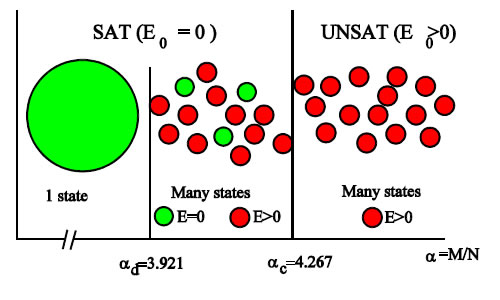
\includegraphics[width=.7\columnwidth]{phase_chart}
\caption{Phase chart for random $\ksat$}
\label{fig:phase_chart}
\end{figure}

\begin{theorem}
For $0 < \d < 1/3$ and $r = (1-\d) 2^k \log 2$, for all $k > k_0(\d)$, there exist $\a < \b < 1/2$ such that $\sf$ consists of $2^{\e_k n}$, with $\e_k = \d/2 - 3/k^2$, non-empty cluster regions with diameter at most $\a n$ and distance between every pair of regions at least $\b n$.
\label{thm:shatter}
\end{theorem}

We will not prove this theorem here, although we shall satisfy ourselves with a rough calculation without proving the details.

\subsection{Exponentially-many clusters}
\label{ssec:exp_many_clusters}
Note that in Eqn.~\eqref{eqn:ksat_vaniall_second_moment}, $\L_S(\a) = \E[\abs{\sf}]$ with overlap ratio of $\a$. For convenience, we introduce $\bL = \L_S(1-\a)$, i.e., expected number of pairs of solutions at a Hamming distance of $\a n$. The program is as follows: If there exists a $z$ s.t. there are no pairs of assignments at distance $z$, it is an upper bound for the diameter of a cluster. Also, if we can find $\bL <1$ in an interval $(\a, \b)$, it is immediate that $\sf$ can be partitioned into regions (i.e., sets of clusters) with distance at least $\b n$ and diameter at most $\a n$. For a clause $c$ in cluster $C$, let $R(C)$ be assignments with distance at most $\a n$ from C and $B(C)$ be all the assignments with distance at most $\b n$ from $R(C)$. Note that since $\bL < 1$ for $(\a, \b)$, $B(C) \setminus R(C)$ does not have any satisfying assignments, i.e., the size of the ``cluster region'' is $\a n$ and the distance between any two regions is at least $\b n$.

We now show that there are exponentially-many such regions. From Sec.~\ref{ssec:ksat_weighted}, we have $\E[X^2] < C \max_{\a \in [0,1]} \L_w(\a)^n$ and since from the second moment method gives $\E[X^2] < C \E[X]^2$, we use the Payley-Zigmund inequality for $t \leq \E[X]$ to get
$$
\P(X > t) \geq \f{(\E[X]-t)^2}{\E[X^2]}.
$$
Take $t = \E[X]/poly(n)$ and see that $X$ is within a polynomial factor of its expectation, i.e., $\L_w(1/2)^{n/2}$ with constant probability. It turns out that the event ``$F$ has more than $q$ solutions'' has a sharp threshold~\cite{achlioptas2008algorithmic} which implies that for $r < 2^k \log 2 - k$,
$$\abs{\sf} > \L_w(1/2)^{n/2}/poly(n) \quad \trm{w.h.p.}$$

We now divide this by the upper bound of the cluster diameter, let $\D = \inf \cbrac{\a: \bL < 1}$ and
$$g_k = \max_{\a \in [0,\D]}\ \bL(\a,k).$$
The expected
number of pairs of solutions with distance \emph{at most} $\D n$ is then
$B < poly(n)\ g_k^n,$
since $\bL$ is expected pairs at particular distance $\a n$
and there are most $n+1$ distances. By Markov's inequality, this means that w.h.p. the number of pairs of solutions at dist. $\D n$ is $poly(n) g_k^n$. Since
every region has size at most $\D n$, w.h.p. the number of pairs in each region is $poly(n) g_k^n$. and if we can show that $g_k < \L_w(1/2)$ we can
see that $\sf$ has at least
$$
\f{1}{poly(n)}\ \rbrac{\f{\L_w(1/2)}{g_k}}^{n/2}
$$
clusters. The rest of the argument then shows that this happens for $\a = 1/k$ and $\b = 1/2 - 5/6\sqrt{\d}$ in Thm.~\ref{thm:shatter}. We do not discuss it here because it is just careful arithmetic, the case for $k > 15$ is analytical and $15 \geq k \geq 8$ is computational. Let us however note that Thm.~\ref{thm:shatter} is quite illuminative, as $r$ approaches the threshold $2^k \log 2$, the clusters are maximally far apart, in fact their size $1/k$ decreases and they vanish as soon as we cross this threshold. Fig.~\ref{fig:phase_chart} shows this phase transition phenomenon for 3-$\SAT$.

Let us note that, using the results in this section, we can show~\cite{achlioptas2008algorithmic} that there exists a $\e_k \to 0$ s.t. the ``glassy'' phase with exponentially-many clusters exists for
$$
(1 +\e_k) \f{2^k}{k} \log 2 \leq r \leq (1-\e_k)\ 2^k \log 2.
$$

\subsection{Survey propagation}
\label{ssec:survey_propagation}

As we saw in Sec.~\ref{ssec:exp_many_clusters}, the solution space of $\ksat$ near the transition threshold lies in the ``error coding regime'' or the ``glassy'' phase, i.e., it consists of exponentially many clusters with exponentially few solutions in each cluster. Note that, random $\ksat$ is not a hard problem per se, below the dynamical transition threshold, exponentially many solutions exist. It turns out that local algorithms based on belief propagation (BP), warning propagation (WP) etc. work well when there are short-range correlations among variables in the factor graph in SAT. Roughly, assumes that the variables in a clause are uncorrelated if that clause is removed (this is true only for trees). This is true only in the ``giant ball'' phase before dynamical phase transition.

On the other hand, as shown in~\cite{achlioptas2006solution}, a large fraction of variables in every cluster region are ``frozen'', i.e., they take the same value for all the satisfying assignments in the cluster. Moreover, they correlate strongly with values of frozen variables in neighboring clusters, which is why message passing algorithms on the random factor graph do not work well.

Survey propagation (SP)~\cite{braunstein2005survey} then, is an algorithm based on the cavity method from statistical physics. Roughly, it sends a warning message (i.e., $\mu^\a(a, i) = 1$) from a factor $a$ to a variable $i$, if all the satisfying assignments of some cluster region $\a$ are such that they do not satisfy $a$, in other words, variable $i$ has the complete responsibility of satisfying $a$. Every cluster region is picked with a probability proportional to the number of satisfying assignments in it. SP therefore hinges on explicitly introducing long-range correlations among different cluster regions. This method is also known as 1-step replica symmetry breaking in statistical physics.

\section{Summary}
\label{sec:summary}

This project discussed phase transition phenomenon in the solution space of random satisfiability problems. We derived bounds for the satisfiability transition threshold using the first and second moment methods for random 2$\SAT$ and $\ksat$. We also briefly explored the phenomenon of dynamical phase transition, wherein the solution space changes drastically and bifurcates into exponentially many clusters. This was used to discuss survey propagation that is one of the state-of-the-art solvers for random satisfiability problems.


{
\small
\bibliography{writeup}
\bibliographystyle{alpha}
}
\end{document}
